

\section{Channel File 291 Incident}
\label{sec:crowd}

Friday July 19, 2024, CrowdStrike, a leading cybersecurity firm, released an update to its Falcon Sensor
software designed for Windows-based systems. The update, intending to enhance threat detection, single-handedly
disrupted the global IT infrastructure, causing widespread system crashes across various industries
(e.g., airlines, healthcare, and banking) \cite{crowdstrike2024falcon}.

The outage costed fortune \textbf{500 companies approximately \$5.4 billion} in damages, after an
estimated \textbf{8.5 million devices} were struck by the blue screen of death (BSoD) \cite{tidy_crowdstrike_outage_2024}\cite{kerner_crowdstrike_outage_2024}.

\section{Context and Background}
\label{sec:context}

CrowdStrike's Founder and CEO George Kurtz, addressed the public on live TV, stating ``That we're deeply sorry for the impact we've caused'' \cite{sato_crowdstrike_ceo_2024}.
Though this isn't the first time George Kurtz has been caught in the crossfire of a cybersecurity incident.
In 2010, George Kurts was the Executive Vice President and Chief Technology Officer at McAfee when they released a faulty update, also causing a BSoD
The update, mistakenly identified a critical Windows system file (svchost.exe) as malware, causing the system to endlessly loop \cite{volenik_crowdstrike_ceo_2024}.

In a blog posted by CrowdSTrike ``as of 8:00 p.m. EDT on July 29, 2024, ~99\% of Windows sensors were back online'' \cite{crowdstrike_channel_file_291_2024}.
The incident occurred due to a bug which expected 20 input fields instead of 21, causing the software to crash. Channel File 291 was identified as the
culprit and was removed from the software \cite{crowdstrike_channel_file_291_2024}.

\section{Modern Endpoint Security}
\label{sec:falcon}

CrowdStrike, as a cybersecurity company, offers endpoint security in the form of their Falcon solution. Falcon is a lightweight agent installed on endpoint devices to monitor and record system activity.
Securing \textbf{endpoints} means securing devices that connect to a network, such as laptops, desktops, and mobile devices, and thus, this is known as \textbf{endpoint security}.
90\% of successful breaches and 70\% of data breaches originate at an endpoint, costing companies millions \cite{ibm_endpoint_security}.
Since many large scale companies have moved to the cloud, and many employees are working from home, ever more devices are connecting to sensitive data. This means many endpoint solutions
have to constantly monitor and record system activity to detect and prevent threats. This in itself utilizes cloud-based systems to access threat intelligence, providing autonomous
real-time protection \cite{cisco_endpoint_security}

Many original anti-viruses signature based, protecting endpoints on a device by scanning for known malware---\textbf{Indicators of Attack (IOA)}.
This relied on a database of known malware signatures. CrowdStrike and many others
have opted to use \textbf{next-gen anti-virus (NGAV)} machine learning technology,
to aid in detecting newer types of IOA vectors that are often fileless, by monitoring system memory  \cite{ionescu_kernel_access_2024}.

\newpage

\section{EPP \& EDR Anti-virus Solutions}
\textbf{Endpoint Protection Platforms (EPP)} like CrowdStrike may include the following features as defined by IBM \cite{ibm_endpoint_security}:
\begin{itemize}
    \item \textbf{Web control and content filtering}: protects against malicious code in websites and
          user downloaded content. While providing a whitelist of approved websites.
    \item \textbf{Data classification and data loss prevention (DLP)}: identifies and classifies sensitive data,
          preventing unauthorized access and data loss.
    \item \textbf{Firewall}: monitors and controls incoming and outgoing network traffic based on configured security rules.
    \item \textbf{Email Gateway}: scans incoming email attachments and links for malicious content.
    \item \textbf{Application control}: restricts the programs that users can run on their devices.
\end{itemize}

CrowdStrike's \textbf{Endpoint Detection and Response (EDR)} solution Falcon Sensor, part of the Falcon Platform, is at the root of the issue.
EDRs are a class of security tools that go beyond known threats, to monitor files entering and applications running on a system.
These \textbf{Correlate Indicators of Compromise (IOC)} systems, aggregate data from various sources---network traffic, unusual user behavior,
inconsistent permissions, system configuration changes, unverified software or domains, repetitive file access, and more \cite{microsoft_ioc}.

These systems aren't just designed to detect threats, but respond to them while an attack is in progress. This incurs IOCs many log based solutions such as
\textbf{extended detection and response (XDR)}, and \textbf{security information and event management (SIEM)} systems to mitigate and isolate threats, going
as far as to shut down a system if necessary. These systems typically rely on AI to establish a baseline of normal activity and detect deviations from it \cite{microsoft_ioc}.

\section{CrowdStrike Falcon Sensor Distinctions}

The immediate reason why CrowdStrike's Falcon Sensor update caused such a widespread outage was due to
the software living on at kernel level. These differ from traditional user-mode applications that crash in isolation.
Kernel-level applications are more privileged living at the heart of the operating system---if it crashes, the whole system crashes.
This process is known as \textbf{kernel panic}, which stops the system from potentially corrupting beyond repair \cite{awati_kernel_panic}.

CrowdStrike notes three main kernel-level component features that it complies with from the Microsoft's anti-virus kernel APIs \cite{ionescu_kernel_access_2024}:
\begin{itemize}
    \item \textbf{Kernel Patch Protection (KPP)}: also known as \textbf{PatchGuard}, prevents third-party software from modifying the Windows kernel.
          Available on 64-bit (x64) Window systems, but by-passable on 32-bit (x86) systems, CrowdStrike opts to never patch the kernel. Other
          anti-virus choose this route, which can lead to system instability if not done correctly \cite{wikipedia_kpp}.
    \item \textbf{Kernel-Mode Code Signing (KMCS)}: CrowdStrike complies with Microsoft's KMCS requirements, which ensures that all kernel-mode code obtains a
          \textbf{Extended Validation (EV) Code Signing Certificate} from a trusted \textbf{Certificate Authority (CA)} \cite{microsoft_kmcs}\cite{reasonlabs_kernel_hooking}.
    \item \textbf{Object Callbacks:} a feature that allows CrowdStrike to subscribe to various kernel events, such as file creation, registry access, and network activity.
          Instead of \textbf{kernel hooking}, which intercepts system calls \cite{microsoft_obregistercallbacks}.
\end{itemize}

CrowdStrike further justifies its kernel presence to protect against for \textbf{Early Boot Protection (EBP)} and which
Microsoft supports with its \textbf{Early Launch Anti-Malware (ELAM)} driver \cite{ionescu_kernel_access_2024}. This protects against rootkits, which are
malware that can hide from the operating system, by loading before the operating system itself. Having this
protection in place, stops attackers from sticking USBs into airport kiosks or hotel computers \cite{baker_rootkits_2023}.

\section{Faulty Code and Production Updates:}

Despite CrowdStrike Falcon Sensor passing \textbf{Windows Hardware Compatibility Program (WHCP)} certifications, and
validations through \textbf{Windows Hardware Lab Kit (HLK)} testing, the update still slipped through \cite{microsoftwhcpcertification}.
However, anti-virus software only needs to pass the WHCP and HLK tests once. They only certify that the driver running on the system
is stable. Once the driver is installed, CrowdStrike can push updates---\textbf{without re-certification}---in a cloud-based process they call
\textbf{Rapid Response Content (RRC)} \cite{crowdstrikechannelfile291rca}.

This process entirely relies on CrowdStrike's internal deploy and testing pipelines. CrowdStrike's testing negligence, did not thoroughly test the update,
during their RRC update to its Falcon Sensor software. Typically a software companies employ \textbf{Continuous Integration/Continuous Deployment (CI/CD)} pipelines
to catch these issues. CI/CD pipelines are characterized by multiple rounds of manual written tests, peer reviewed code, and automated stress testing to ensure the software compiles safely before deployment \cite{redhat_cicd_2023}.
These tests comprise of \textbf{unit tests}, \textbf{integration tests}, and \textbf{end-to-end (E2E) tests} to ensure the software is functioning as expected.
Unit tests test individual components of the software, integration tests test how the components interact, and E2E, running the application in production-like environments (e.g., test and development environments before production) in
a suite of integration tests to ensure stability. CrowdStrike lacked the CI/CD security to catch Channel File 291, a bug that effectively threw an out-of-bounds error.

\section{CrowdStrike Incident Report}

Before jumping into CrowdStrike's incident analysis, we must first understand the technical terms used in the analysis \cite{crowdstrikechannelfile291rca}:

\begin{enumerate}
    \item \textbf{Falcon OverWatch\textsuperscript{\textregistered} and Falcon Complete\textsuperscript{\texttrademark}}: OverWatch is a 24/7 managed threat hunting service led by human
          intelligence. Complete is a \textbf{managed detection and response (MDR)} service, which is a suite of tools and services including OverWatch, to detect and remediate threats
          \cite{cosive_falcon_complete}\cite{crowdstrike_falcon_complete}\cite{crowdstrike_overwatch}.

    \item \textbf{Security Telemetry \& Graph Store}: Telemetry is the aggregation of data from various sources (e.g., endpoints, servers, network devices) \cite{proofpoint_telemetry}. These analytics are
          are stored locally on the Falcon Sensor's sensors in a graph database. Graph databases store information in nodes and edges to represent
          the relationship between data points \cite{oracle_graph_database}.

          \newpage
          Falcon Sensor's interprets relationships in flowing memory to detect possible IOAs.\\
          \begin{figure}[h!]
              \vspace{-1em}
              \centering
              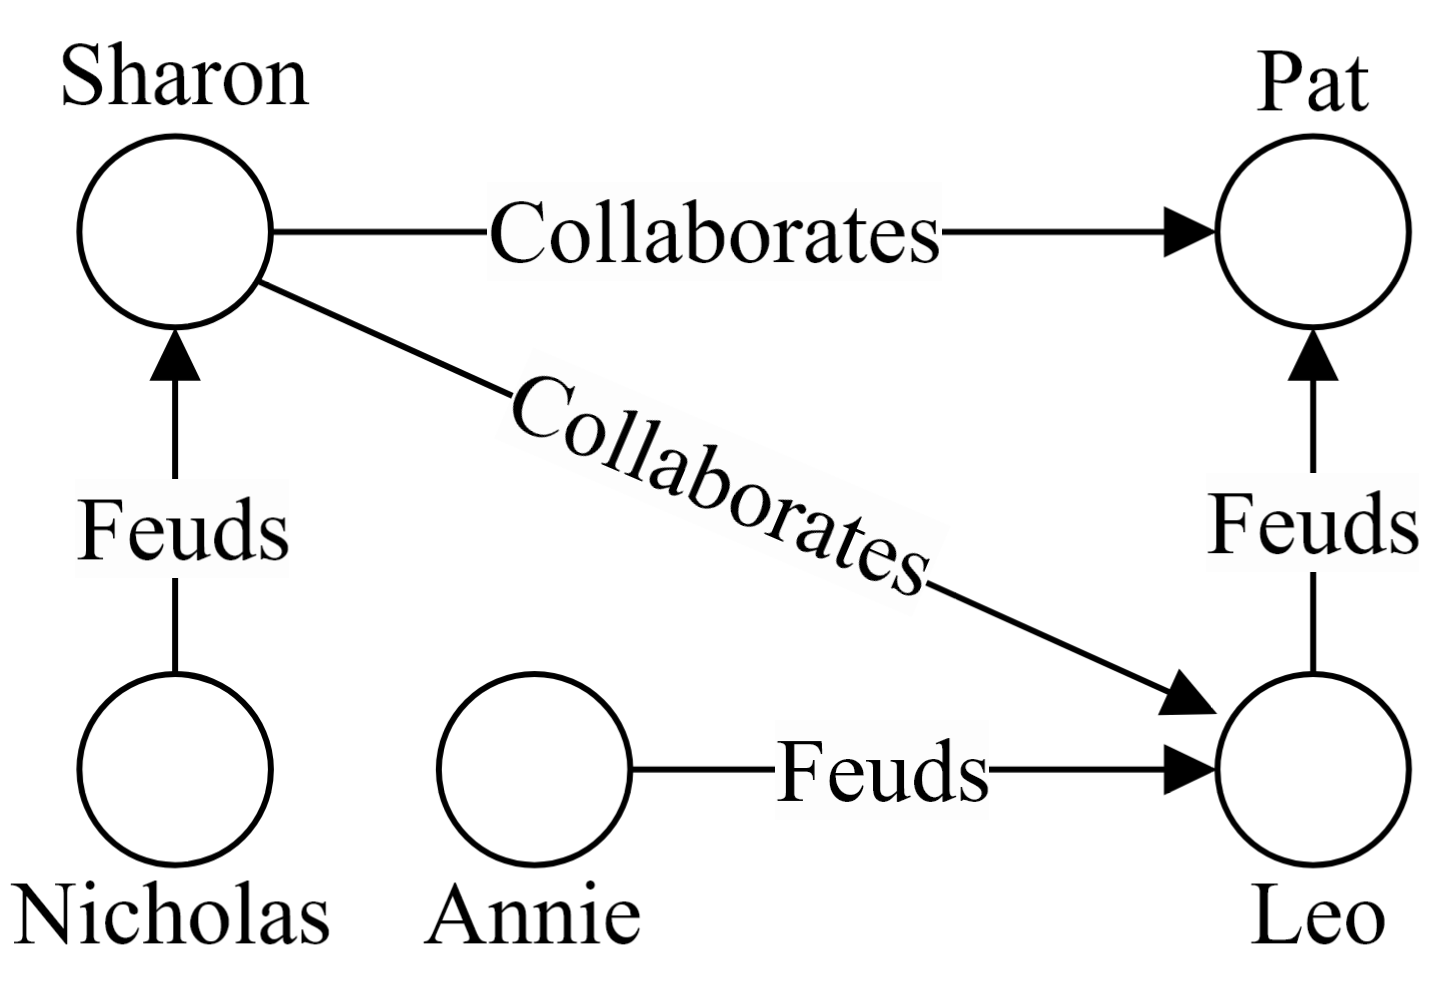
\includegraphics[width=0.35\textwidth]{Sections/crowd/graph.png}
              \caption{Graph Example Depicting Relationships Between Co-workers}
              \label{fig:graphdb}

              \vspace{-1em}
          \end{figure}

    \item \textbf{Template Types}: Template types push telemetry data to a regular-expression (RegEx) engine
          Content Interpreter. Template types outline predefined schemas of security criteria to evaluate. \textbf{Template Instances}
          are live configurations, defining parameters, thresholds, and conditions to trigger alerts.
    \item \textbf{Channel Files}: Each Falcon sensor defines a channel file, which is configured with a
          template type. RRCs then push threat intelligence to channel files. Template instances then compare the security telemetry to
          determine IOAs.


          \begin{figure}[h!]
              \centering
              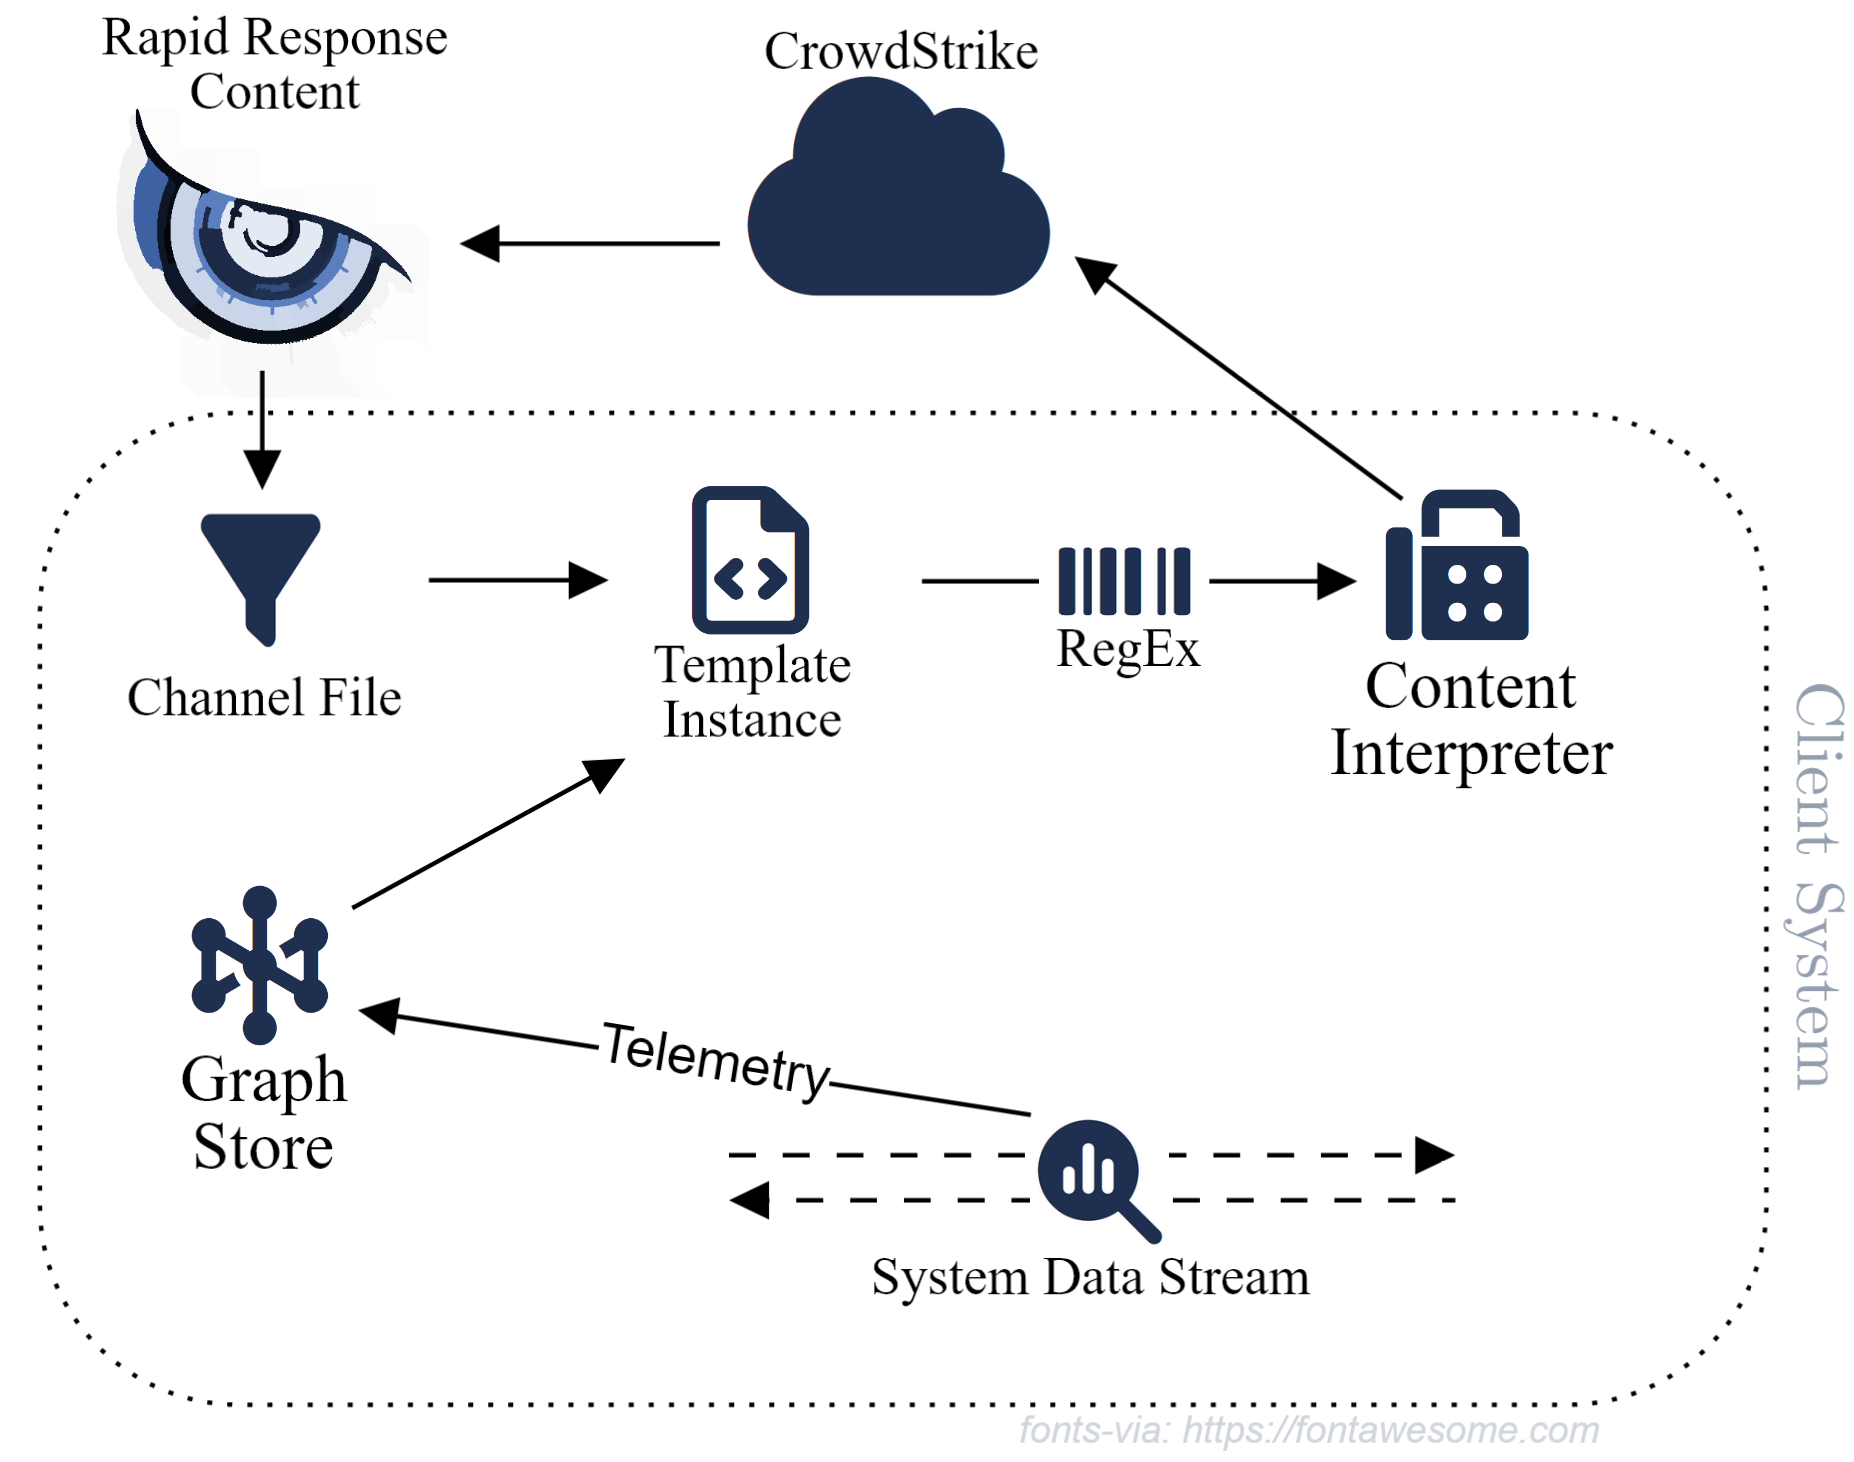
\includegraphics[width=.65\textwidth]{Sections/crowd/rrc.png}
              \caption{RRC \& Telemetry Graph Store Data Aggregation for IOA Content Interpreter.}
              \label{fig:channelfile}
          \end{figure}
\end{enumerate}

\vspace{-1em}
February 2024, CrowdStrike released sensor version 7.11, introducing a new template type.
The template type target a new IOA vector relating to \textbf{Windows Interprocess Communication (IPC)} mechanisms---notably \textbf{Named Pipes}.
Named pipes facilitate communication between processes on the same or different machines.
The exploit enabled an adversary to execute code and impersonation leading to privilege escalation \cite{sandker_named_pipes_2021}.

This release included a new IPC template type. RRC delivers IPC template instances to \textbf{Channel File 291}. This
new template type defined 21 input fields, while the Content Interpreter still expected 20. This evaded detection
as the Content Interpreter identified files based on a wildcard matching pattern.

\begin{lstlisting}[caption=Wildcard Pattern Matching Example]
    *: Matches any sequence 
    ?: Matches any single character
    Input: txt = ``abcdef'', pattern = ``a?c*''
    Output: true
    Reason: `?' matches with `b' and `*' matches with ``def''.
\end{lstlisting}

\noindent
(As CrowdStrike has mentioned their use of RegEx before, it is likely that the Content Interpreter used a RegEx pattern to match fields.)

On July 19, 2024, the RRC push two new IPC template instances to Channel---one of which dropped wildcard matching.
This required the Content Interpreter to check the 21st field from Channel File 291. However, the Content Interpreter
expected 20 fields, causing an out-of-bounds error, crashing the Falcon Sensor. This error
caused the BSoD that Friday afternoon affecting 8.5 million devices.

\section{Windows Kernel Crash Dump Analysis}

David Weston, Vice President, Enterprise and OS Security at Microsoft, \href{https://www.microsoft.com/en-us/security/blog/2024/07/27/windows-security-best-practices-for-integrating-and-managing-security-tools/}{posted} in an incident
the kernel crash dump from Channel File 291 \cite{weston_windows_security_2024}. The Microsoft team's \textbf{Windows Error Reporting (WER)}
kernel crash dumps analysis involved \textbf{WinDBG Kernel Debugger}, and several other freely accessible debugging extensions.

\begin{figure}[h!]
    \centering
    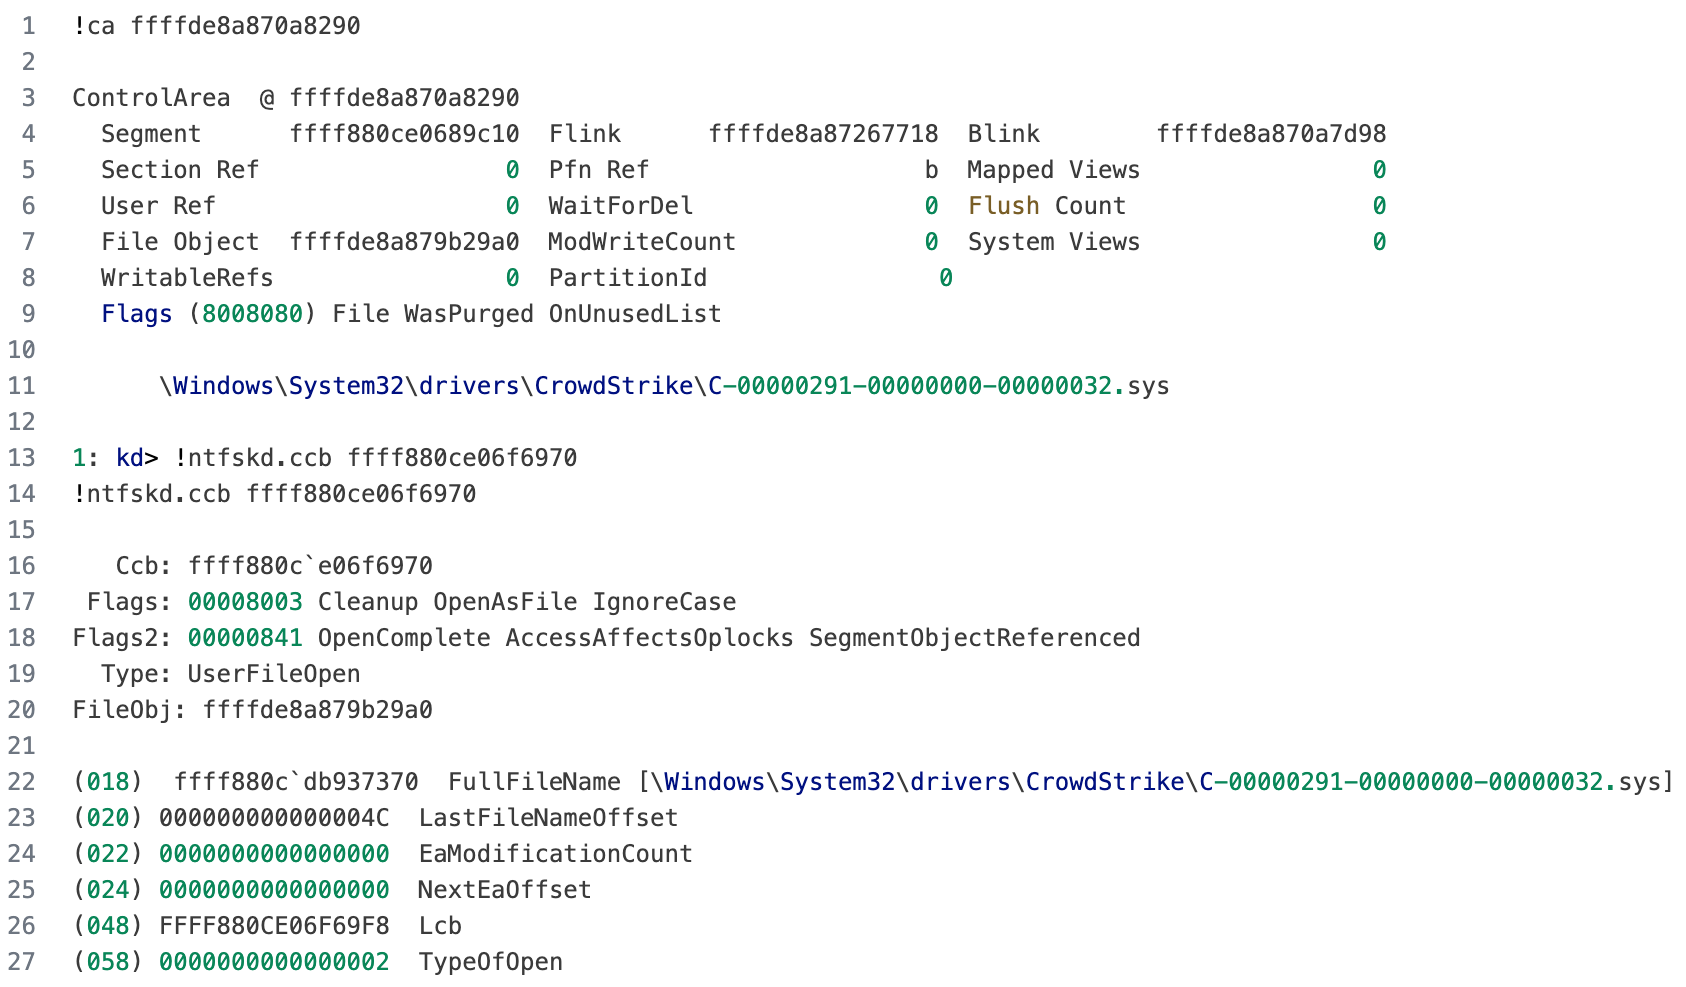
\includegraphics[width=1\textwidth]{Sections/crowd/fig1.png}
    \caption{Channel File 291 Incident Analysis}
    \label{fig:fig1}
\end{figure}

\noindent

\noindent
Line 23 (modified to fit page) shows the full file path of Channel File 291, confirming the cause of the crash.
The dump shows the crash is due to an out-of-bounds error.
While the crash dump is not publicly available, the Microsoft team confirms the out-of-bounds error in the given crash dump.
Microsoft confirmed the crash to be Crowdstrike's fault early on into the incident due to there being no public facing crash message, only a BSoD, which led to some to believe Microsoft was at fault.

Despite the fact that this is not Kurtz's first significant security mishap, it would be unfair to place responsibility squarely on his shoulders:
each Windows sensor release is certified through extensive testing in Microsoft's HLK and WHQL.
The lack of comprehensive end-to-end testing introduced a critical error that was not caught by their CI pipelines. Such an erroneous
mistake could have been easily caught in a test or development environments, raising substantial concerns.
The 12 page incident report duly noted this, mentioning under point 5 of the Findings and mitigations section that CrowdStrike should
"expand [validation] to include testing within the Content Interpreter" \cite{crowdstrikechannelfile291rca}.
Even though customers managed to recover from the incident, but CrowdStrike continues to face severe legal repercussions.

\section{Legal Issues Raised by CrowdStrike Outage}
These critical lapses in CrowdStrike's CI/CD practices has led to significant legal repercussions including a \$500 million dollar lawsuit
filed by Delta Airlines. 
The lawsuit alleges that CrowdStrike's negligence in testing and deploying the update caused the outage.
However, it is likely that CrowdStrike will walk away from this lawsuit scott-free, as Delta's stance of CrowdStrike's breach of contract and negligence will be
extremely difficult to prove in court. CrowdStrike's faulty code and production updates may be deemed as not convincing enough to hold them accountable for the damages caused by the outage.
"It's one thing to claim faulty software caused an outage, he says, but another to prove Crowdstrike didn’t take adequate precautions on testing or monitoring", claimed liability lawyer Ramzy Ladah.
\cite{delta_lose} At this point, it seems likely that Delta will lose the lawsuit, as CrowdStrike's negligence in testing and deploying the update will be difficult to prove in court.


Delta's lawsuit won't be the only legal repurcussion that CrowdStrike will face. They are to face a class-action lawsuit from the 8.5 million devices that were affected by the outage as well. Moving past
the actual legal repurcussions, it is interesting to see that for the scope of the outage, CrowdStrike has not faced any legal repurcussions from the government. In contrast, Snowflake, an AI cloud-based data company,
was subject to an investigation by the SEC for its cyber breach that posed the threat of data leakage. \cite{snowflake_sec} This raises the question of why CrowdStrike has not faced any legal repurcussions from the government despite
its severity of the outage. This could be due to the fact that Snowflake had issues regarding the mismanagement of customer data in contrast to CrowdStrike's incident while damaging,
did not pose a threat to the data of its customers.


However, an important point to make notice of, is the fact that CEO George Kurtz has been in a similar situation before with McAfee. Considering the frequency of
vulernabilities like this, there must be an industry/government standard that companies should adhere to.  While some frameworks, such as ISO 27001, exist to guide organizations in securing their information systems,
there is no universally mandated standard specifically addressing the testing, deployment, and monitoring practices in CI/CD pipelines. This lack of regulation allows companies to cut corners around the thorough testing required to ensure security and stability.
It is vital that the United States adheres to a standard, such as the EU's NIS2 Directive that requires companies to meet minimum benchmarks.
Some of these benchmarks include rigorous pre-deployment testing and third-party audits. \cite{eu_nis2} Initiatives like this is what keeps companies in the EU above standard,
and until now there have not been any publicly reported cases of companies facing fines under the NIS2 Directive. This is a testament to the effectiveness of the NIS2 Directive in ensuring that companies adhere to a standard that protects their customers.
Considering this, the United States must follow suit such that we can prevent incidents like CrowdStrike's outage from happening in the future. Aside from the legal aspects of CrowdStrike, there are also various ethical issues that arose from the outage to consider.

\section{Ethical Issues Raised by CrowdStrike Outage}

The scale of the CrowdStrike outage is only matched by the outrageousness of the mistake. Public opinion is divided on how to feel about the issue. Some consumers wonder how a giant corporation could have let such a mistake occur, while others take comfort in the fact that it was only a mistake that could be fixed and not a deliberate attack that could have had more devastating consequences.  Ethical questions have arisen as a result.

CrowdStrike provides 25 percent of all enterprise endpoint solutions and has both immense power and responsibility in the cybersecurity space. Following the outage, on September 24th CrowdStrike’s Senior VP of Counter Adversary Operations, Adam Meyers, was called to testify in front of the House Homeland Security Subcommittee on Cybersecurity and Infrastructure Protection. The one-and-a-half-hour hearing underlines the connective-ness between CrowdStrike and governmental institutions and regulatory bodies. Most people wonder if more is necessary.

The startling fact that the error could have been easily detected if the update was run on a secured machine before deployment led to the joke of "testing in production" in the coding space. When consumers expect a company to provide them with a product, they also expect the product to not break as a result of the provider's mistakes. This highlights the issue of consumer trust and confidence in a space where products are proprietary and consumers have very little understanding of the actual moving parts in the products they are purchasing or how they are maintained.

Should the public, as consumers, have to simply trust private enterprises to properly maintain their products and uphold their commitments, or should more control and oversight be put upon them, and is that even possible? It raises the question of whether a government can even provide meaningful oversight that doesn't interfere with a company's development or trample user rights. This train of thought only seems to lead to a loss of consumer confidence.

Another issue is the fact that we had to learn about this error in CrowdStrikes CI/CD pipeline and deployment practices as a result of experience. At the very minimum consumers expect regulatory bodies to have methods and procedures in place to either prevent or spot these errors before they even can affect the real world. An example would be similar to OSHA, which people trust to enforce worker protections and safe practices in the construction space. Now, people are asking where was an OSHA equivalent in the case of preventing the CrowdStrike outage.

In some cases, that already exists in the US with CISA, or the Cybersecurity and Infrastructure Security Agency. A federal agency that is the "operational lead for federal cybersecurity and the national coordinator for critical infrastructure security and resilience". CISA was the federal head of response to the CrowdStrike outage. But why weren't they able to prevent such an outage from occurring in the first place, and why aren't there repercussions on CrowdStrike as a response?

In a statement about the outage CISA Director Jen Easterly called it a "terrible incident" but also "a useful exercise, like a dress rehearsal for what China may want to do to us." This response and subsequent discussion highlighted that the Director was more focused on moving past the incident entirely and more on how it prepared the agency and industry as a whole for the outcomes of the outage. Entirely missing is the fact of how a mistake like this occurred in the first place.

CISA understands the implications of the outage but also understands the position of CrowdStrike in the cybersecurity space. All of this shows that CISA and the US government are satisfied with simply holding a Congressional hearing and receiving CrowdStrike's incident report, which is federally mandated by the Cyber Incident Reporting for Critical Infrastructure Act of 2022. It would not be out of place to say that the US government understands the position and power of CrowdStrike and as such, cannot take drastic public measures that would drag CrowdStrike's name through the mud and degrade confidence in the company as a whole and the Falcon Sensor as a product. It is somewhat mutually beneficial to leave it at a "do better next time" which preserves the image of CrowdStrike while letting them continue selling a very critical and in-demand product.

Another side issue is the responsibility of Microsoft in all of this. As CrowdStrike deploys its updates to Windows machines through Microsoft, where was their due diligence in the matter? As stated before, Microsoft only certifies the necessary software and drivers once, to make sure they run without difficulties the first time around. Should this have to change as cyber-security software often requires constant communication between cloud-based resources and the driver located on the Windows Kernel? Can Microsoft even be expected to re-certify every update that a third-party vendor intends to push?

In September Microsoft hosted a Windows Endpoint Security Ecosystem Summit on the topic of endpoint security attended by multiple security vendors from the Microsoft Virus Initiative (MVI) as well as government officials from the United States and the European Union. Microsoft has stated that they intend to present more options to vendors for security outside of the kernel and has proposed kernel access restrictions to third parties to permanently avoid issues similar to the Crowdstrike outage from occurring.

As draconian as this might sound, it is a rock-solid solution as Microsoft wouldn't need to potentially re-certify the constant updates required in the ever-evolving cyber-security space. However, this leads to the deduction that Microsoft wants more control over the Windows OS and Kernel as it is related to security. If only Microsoft had access to the Windows Kernel, they would be at a marked advantage over other security vendors that would have to "work from the outside".

Some conclusions have been gained from all of this. Microsoft has endeavored to expand non-kernel measures for vendors, decreasing the likelihood of faulty code resulting in BSoD's. Increasing awareness has been garnered in the CI/CD and deployment practices of cyber-security vendors, especially those with kernel-level access. Hopefully, this awareness will lead to standardized practices and government enforcement and oversight that will prevent significant mistakes that lead to the CrowdStrike outage.